\chapter{Optimization of truss structures}
In this chapter, we focus on the optimization of discrete truss structures. A general procedure to solve such problems involves the following steps:
\begin{enumerate}
    \item Definition of the truss with all nodes, elements, material properties, constraints and initial design choice
    \item Solution of unknown displacements for each node in the truss given the current design
    \item Evaluation of the objective function and its gradients w.r.t. the design variables
    \item Approximation of the problem with MMA at the current design point
    \item Solution of the approximated dual problem to find the next design point
    \item Repetition of steps 2,3,4 and 5 until a maximum of iterations is reached or until there is no improvement of the objective function any more
\end{enumerate}


\begin{objectives}{}{objectives_shape}
After studying this chapter and finishing the exercise, you should be able to 
\begin{itemize}[label=$\dots$]
    \item define optimization problems to minimize compliance of two-dimensional trusses with a volume constraint
    \item explain properties of the aforementioned optimization problem
    \item employ MMA to solve two-dimensional truss optimization problems
\end{itemize}
\end{objectives}

\section{Size Optimization}
One possible objective in truss optimization is the search for the cross sectional areas $\mathbf{a}$ resulting in the stiffest truss. The corresponding objective function could be simply the displacement at a specific node or a global displacement measure $\mathbf{u} (\mathbf{a}) \cdot \mathbf{u} (\mathbf{a})$. However, we choose to minimize the compliance $C: \mathcal{R}^{M} \rightarrow \mathcal{R}$ defined as 
\begin{equation}
    C(\mathbf{a}) = \mathbf{f} \cdot \mathbf{u}(\mathbf{a})
\end{equation} 
of the truss instead. The minimal compliance results also in the stiffest truss, but this formulation is preferred over the pure displacement formulation, because $C(\mathbf{a})$ is convex \cite{Svanberg1984}. The convexity is proven by showing that the Hessian $\nabla^2 C(\mathbf{a})$ is positive semi-definite, a property that is inherited from the positive semi-definiteness of $\mathbf{K}(\mathbf{a})$ (see Chapter 5.2.1 in \cite{Christensen2008} for details).

We employ box constraints $\mathcal{A}$ on the upper and lower limit of the design variables. The upper limit $\mathbf{a}^+$ could be a manufacturing constraint that prevents very thick elements. The lower limit $\mathbf{a}^-$ should be larger than $0$ to prevent deletion of truss elements. If the cross sectional area of all elements connected to a node would become $0$, i.e. all trusses are deleted, the displacement of that node would be undetermined and the stiffness matrix would become singular. In this chapter, we prevent this by demanding $a_j- > 0$.

A typical inequality constraint is a volume constraint for the total truss volume used in the assembly. If we would not have a volume constraint, the optimization would predict a trivial solution with all cross sections at their maximum area. However, we are interested in solutions that put a limited material resource to its best use and thus limit the total volume to be 
\begin{equation}
    \mathbf{a} \cdot \mathbf{l} \le V_0
\end{equation}
where $V_0$ describes the maximum volume used in the design
In order to find a solution at all, we must obviously choose $V_0 \ge \mathbf{a}^- \cdot \mathbf{l}$, otherwise it would be impossible to find any $\mathbf{a}$ fulfilling the constraint. 

In conclusion, the size optimization problem for a stiff truss with limited volume may be noted as follows:

\begin{equation}
    \begin{aligned}
        \min_{\mathbf{a}} \quad & C(\mathbf{a}) = \mathbf{f} \cdot \mathbf{u}(\mathbf{a})\\
        \textrm{s.t.} \quad & \mathbf{a} \cdot \mathbf{l} - V_0 \le 0  \\
                            & \mathbf{a} \in \mathcal{A}\\
    \end{aligned}
    \label{eq:size_optimization}
\end{equation}

The objective function $C(\mathbf{a})$ is convex, the inequality constraint $\mathbf{a} \cdot \mathbf{l} - V_0$ is convex, and the set $\mathcal{A}$ is compact and convex. Therefore, finding a KKT point is equivalent to finding the global unique solution of the problem. We can denote the Lagrangian 
\begin{equation}
    \mathcal{L}(\mathbf{a}, \mu) = C(\mathbf{a}) + \mu \left( \mathbf{a} \cdot \mathbf{l} - V_0 \right) 
\end{equation}
and need to compute the gradient $\frac{\partial \mathcal{L}}{\partial a_j}$ to solve the optimization problem. It is 
\begin{equation}
    \frac{\partial \mathcal{L} (\mathbf{a}, \mu)}{\partial a_j} 
    = \frac{\partial C (\mathbf{a})}{\partial a_j} + \mu l_j
    = \mathbf{f} \cdot \frac{\partial \mathbf{u} (\mathbf{a})}{\partial a_j} + \mu l_j,
    \label{eq:lagrange_truss_problem}
\end{equation}
where the gradient $\frac{\partial \mathbf{u} (\mathbf{a})}{\partial a_j}$ remains to be determined. It can be obtained by differentiating Equation \eqref{eq:global_stiffness} w.r.t $\mathbf{a}$
\begin{align}
        \frac{\partial}{\partial a_j} \mathbf{f} &= \frac{\partial}{\partial a_j} \left( \mathbf{K} (\mathbf{a}) \cdot \mathbf{u} (\mathbf{a}) \right) \\
        0 &= \frac{\partial \mathbf{K} (\mathbf{a})}{\partial a_j} \cdot \mathbf{u} (\mathbf{a}) + \mathbf{K} (\mathbf{a}) \cdot \frac{\partial \mathbf{u} (\mathbf{a})}{\partial a_j}
\end{align}
and rearranging the terms to yield
\begin{equation}
    \frac{\partial \mathbf{u} (\mathbf{a})}{\partial a_j} = - \mathbf{K}^{-1}(\mathbf{a}) \cdot \frac{\partial \mathbf{K} (\mathbf{a})}{\partial a_j}  \cdot \mathbf{u} (\mathbf{a}).
\end{equation}
Substituting this expression into the previous Equation \eqref{eq:lagrange_truss_problem} gives us the sensitivity of the compliance with respect to the design variables 
\begin{align}
    \frac{\partial C (\mathbf{a})}{\partial a_j} 
    &= - \mathbf{f} \cdot \mathbf{K}^{-1}(\mathbf{a}) \cdot \frac{\partial \mathbf{K} (\mathbf{a})}{\partial a_j} \cdot \mathbf{u} (\mathbf{a})  \\
    &= - \mathbf{u} (\mathbf{a}) \cdot \frac{\partial \mathbf{K} (\mathbf{a})}{\partial a_j} \cdot \mathbf{u} (\mathbf{a})  \\
    &= - \mathbf{u}_j (\mathbf{a}) \cdot \frac{\partial \mathbf{k}_j(a_j)}{\partial a_j} \cdot \mathbf{u}_j (\mathbf{a})  \\
    &= - \mathbf{u}_j (\mathbf{a}) \cdot \mathbf{k}^0_j \cdot \mathbf{u}_j (\mathbf{a})  \\
    &= - 2 w_j (\mathbf{a})
    \label{eq:compliance_sensitivity}
\end{align}
with 
\begin{equation}
    \mathbf{k}_j^0 = \frac{E}{l_j}
    \begin{pmatrix}
    \cos{\phi}^2 & \cos{\phi}\sin{\phi} & -\cos{\phi}^2 & -\cos{\phi}\sin{\phi} \\
    \cos{\phi}\sin{\phi} & \sin{\phi}^2 & -\cos{\phi}\sin{\phi} & -\sin{\phi}^2 \\
    -\cos{\phi}^2 & \cos{\phi}\sin{\phi} & \cos{\phi}^2 &\cos{\phi}\sin{\phi} \\
    -\cos{\phi}\sin{\phi} & -\sin{\phi}^2 & \cos{\phi}\sin{\phi} & \sin{\phi}^2 \\
    \end{pmatrix}
\end{equation}
and the strain energy density in each element 
\begin{equation}
    w_j = \frac{1}{2} \mathbf{u}_j (\mathbf{a}) \cdot \mathbf{k}^0_j \cdot \mathbf{u}_j (\mathbf{a}).
    \label{eq:element_strain_energy}
\end{equation}
The strain energy density is always greater or equal to zero due to the positive semi-definiteness of $\mathbf{k}^0_j$.
What we have just done is called a \emph{sensitivity analysis} - we obtained an expression of how much a change of variable $a_j$ contributes to the change of the objective function $\frac{\partial C (\mathbf{a})}{\partial a_j}$. It is very valuable to have an analytical expression of the sensitivity, as solving it numerically via finite differences causes a high computational cost and loss in precision.
Finally, the gradient of the Lagrangian becomes 
\begin{equation}
    \frac{\partial \mathcal{L} (\mathbf{a}, \mu)}{\partial a_j} 
    = - 2 w_j (\mathbf{a}) + \mu l_j
    \label{eq:lagrange_sensitivity}
\end{equation}

If we could solve this expression for $\mathbf{a}^*(\mu)$ at the stationary point of the Lagrangian, we could use Lagrangian duality to compute the solution easily. Unfortunately, the solution is not easy, as $w_j$ depends on the global design $\mathbf{a}$ and not just on the design variable in its element $a_j$. For this reason, we will use MMA to solve the problem.

\begin{example}{Fully stressed design}{mitchellexample}
    We can still learn something about the solution if we consider Equation \eqref{eq:element_strain_energy}. If we substitute it in Equation \eqref{eq:lagrange_sensitivity}, we can write 
    \begin{equation}
        \frac{\partial \mathcal{L} (\mathbf{a}, \mu)}{\partial a_j} = - \frac{S^2_j}{E} l_j + \mu l_j
    \end{equation}
    and conclude that for an optimal point $\mathbf{a}^- < \mathbf{a}^* < \mathbf{a}^+$ with $\mu^*>0$, i.e. the maximum volume $V_0$ is used and box constraints are not reached, all stress magnitudes are identical with
    \begin{equation}
        S_j = \pm \sqrt{\frac{\mu^*}{E}}.
    \end{equation}
    
    This is called a \emph{fully stressed design} and is related to a theorem by Australian engineer A.G.M. Michell published in 1904 \cite{Michell1904}. The theorem states that elements of an optimal truss structure lie along the principal directions of a virtual stress field, such that all of them experience an equal stress magnitude \cite{Arora2019}.
    An example for a Michell truss structure is given in the following picture \cite{Picelli2015}. All truss elements in this design experience the same stress magnitude (either in compression or in tension).
    \begin{center}
        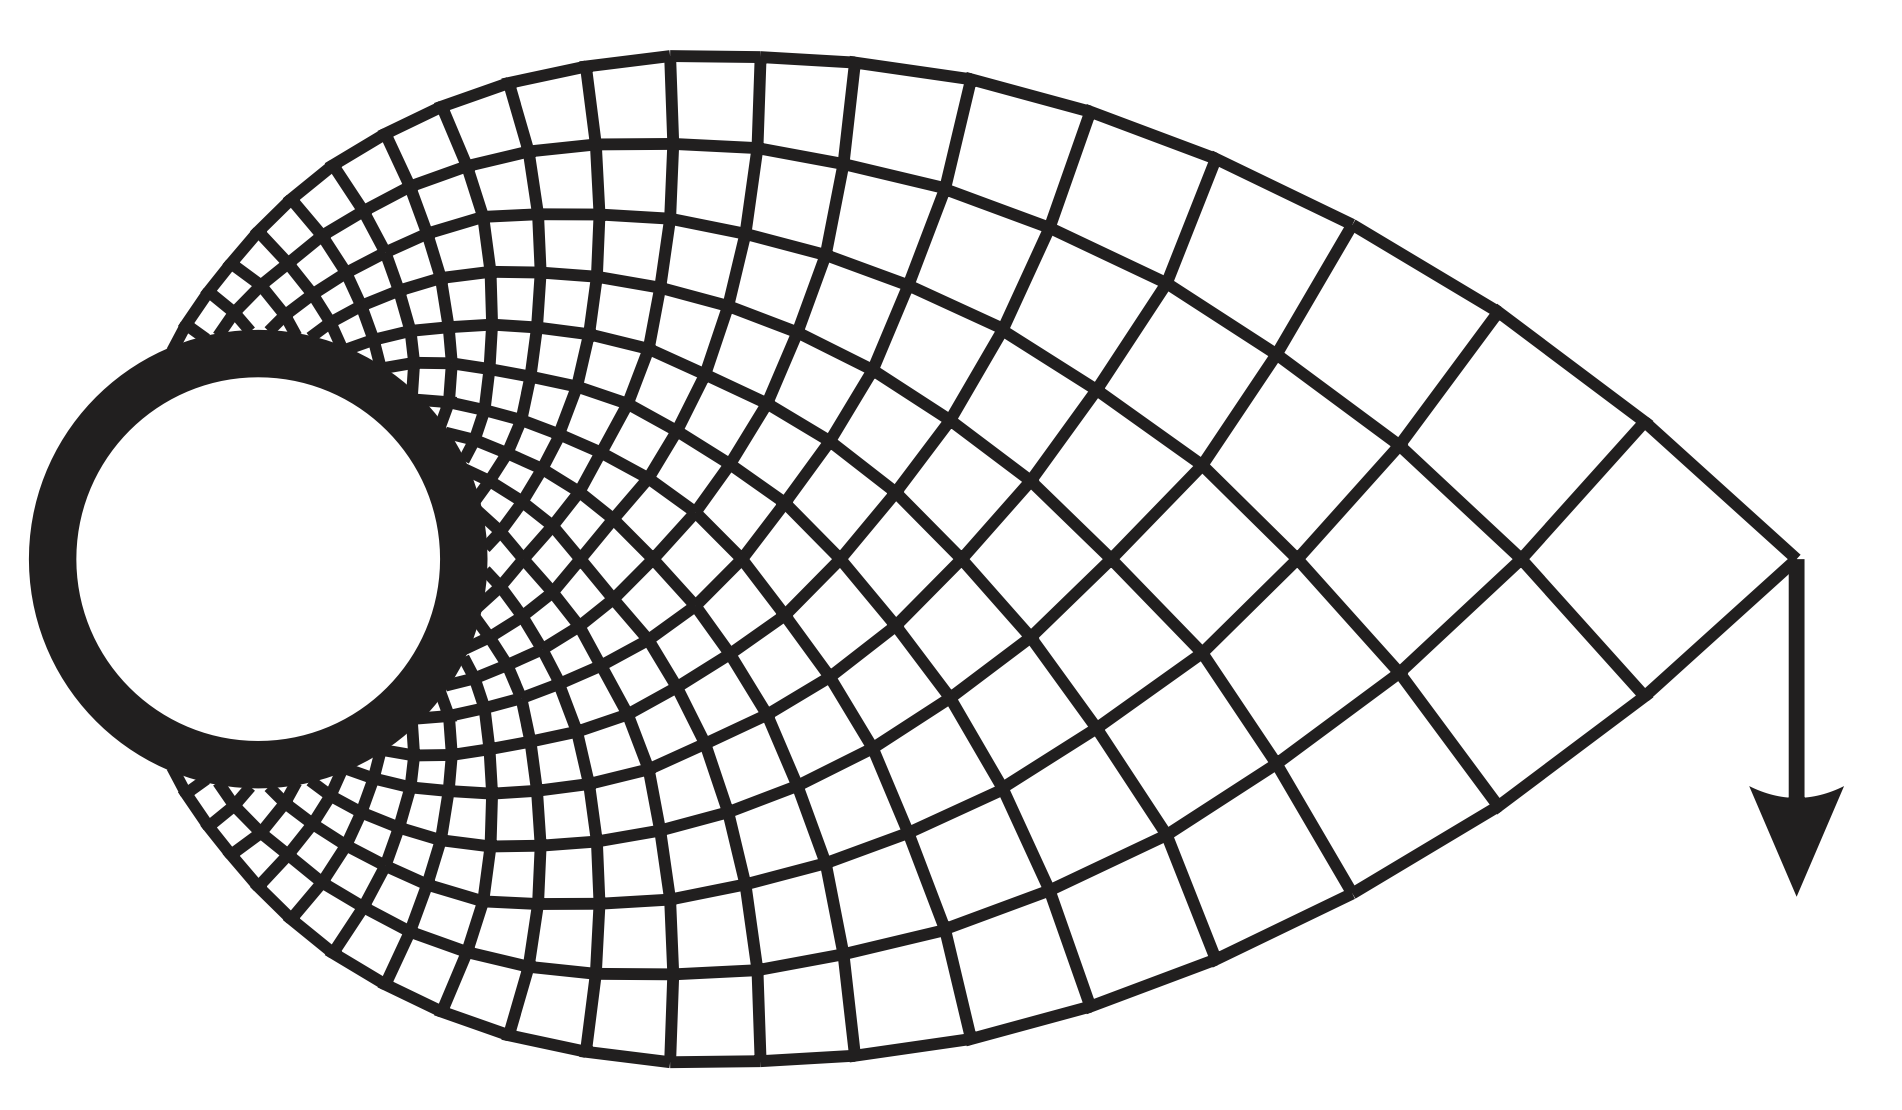
\includegraphics[width=0.5\textwidth]{figures/michell.png}
    \end{center}
    
\end{example}

The problem in Equation \eqref{eq:size_optimization} is convex, but it is not separable and explicit, because we cannot find an explicit expression for $\mathbf{a}^*(\mu)$ at the stationary point of the Lagrangian. Therefore we linearize the problem using MMA in $1/(a_j-L_j^k)$. The linearization of the objective function becomes
\begin{align}
    \tilde{C}(\mathbf{a}) &= C(\mathbf{a}^k) + \sum_j \frac{\partial C}{\partial a_j}(\mathbf{a}^k) (a^k_j-L^k_j) - \sum_j \frac{\partial C}{\partial a_j}(\mathbf{a}^k) \frac{(a^k_j-L^k_j)^2}{a_j-L^k_j}\\
    &=C(\mathbf{a}^k) 
    - \sum_j 2w_j (\mathbf{a}^k) (a^k_j-L^k_j)
    + \sum_j 2w_j (\mathbf{a}^k)
    \frac{(a^k_j-L^k_j)^2}{a_j-L^k_j}.
\end{align}
Note that this is a linearization using lower asymptotes only, because 
\begin{equation}
    \frac{\partial C }{\partial a_j}(\mathbf{a}^k)  = - 2 w_j (\mathbf{a}^k) < 0 \quad \forall \mathbf{a}^k
\end{equation} 
and thus all terms in Equations \eqref{eq:mma_start} and \eqref{eq:mma_end} involving $p_j^k$ vanish.
The approximated optimization problem becomes 
\begin{equation}
    \begin{aligned}
        \min_{\mathbf{a}} \quad & \tilde{C} (\mathbf{a})\\
        \textrm{s.t.} \quad & \mathbf{a} \cdot \mathbf{l} - V_0 \le 0  \\
                            & \tilde{\mathbf{a}}^{-,k} \le \mathbf{a} \le \mathbf{a}^+\\
    \end{aligned}
\end{equation}
with lower move limits $\tilde{\mathbf{a}}^{-,k} = \max(\mathbf{a}^-,  0.9 \mathbf{L}^k + 0.1 \mathbf{a}^k)$ preventing division by zero. The constraint is already linear and thus we do not approximate it.

The Lagrangian of the approximated problem is
\begin{equation}
    \mathcal{L}(\mathbf{a}, \mu) = \tilde{C}(\mathbf{a}) + \mu \left( \mathbf{a} \cdot \mathbf{l} - V_0 \right)
\end{equation}
is separable with 
\begin{equation}
    \begin{split}
        \mathcal{L}(\mathbf{a}, \mu) &= \underbrace{C(\mathbf{a}^k) - \sum_j 2w_j (\mathbf{a}^k) (a^k_j-L^k_j) - \mu V_0}_{\mathcal{L}^0} \\
        &+ \sum_j \underbrace{\left(2 w_j (\mathbf{a}^k)
        \frac{(a^k_j-L^k_j)^2}{a_j-L^k_j} + \mu a_j l_j \right)}_{\mathcal{L}_j (a_j)}.
    \end{split}
\end{equation}
We want to find an explicit expression for $\mathbf{a}^*(\mu)$. Therefore we compute the stationary point of the Lagrangian
\begin{equation}
    \frac{\partial \mathcal{L}_j}{\partial a_j} = -2 w_j (\mathbf{a}^k)
    \frac{(a^k_j-L^k_j)^2}{(\hat{a}_j-L^k_j)^2} + \mu l_j = 0
\end{equation}
and rearrange the equation to find 
\begin{equation}
    \hat{a}_j(\mu) = L_j^k + \sqrt{\frac{2 w_j (\mathbf{a}^k)
    (L^k_j-a^k_j)^2}{\mu l_j}}. 
\end{equation}
We simply clamp this result with box constraints to obtain the explicit relation 
\begin{equation}
    \mathbf{a}^* (\mu) = \textrm{clamp}\left(\hat{\mathbf{a}}(\mu), \tilde{\mathbf{a}}^{-,k}, \mathbf{a}^+\right). 
\end{equation}
Finally we can plug this result in the Lagrangian to get the dual function
\begin{equation}
    \underline{\mathcal{L}}(\mu) = \mathcal{L}(\mathbf{a}^* (\mu), \mu)
\end{equation}
and solve 
\begin{equation}
    \max_{\mu} \underline{\mathcal{L}}(\mu)
\end{equation}
for $\mu^*>0$. This solution procedure is simple - the dual Lagrangian depends only on one variable and the problem is concave. We can use a gradient decent method to solve it quickly and utilize this analytical expression for the gradient 
\begin{equation}
    \frac{\partial \underline{\mathcal{L}}}{\partial \mu}(\mu) =  \mathbf{a}^* (\mu) \cdot \mathbf{l} - V_0.
\end{equation}


\begin{example}{Three bar truss optimization}{trussoptimization example}
    Consider the truss from the previous example. Instead of just computing the displacements, we are now interested in finding the optimal cross sectional areas given a volume constraint.

    We formulate the following algorithm to solve that problem: 
    \begin{enumerate}
        \item Define the truss with all nodes $\mathcal{N}$, elements $\mathcal{E}$, material property $E$, volume constraint $V_0$, design limits $\mathbf{a}^-, \mathbf{a}^+$ and the initial design choice $\mathbf{a}^0$.
        \item Compute the displacements $\mathbf{u}^k = \mathbf{u}(\mathbf{a}^k)$ by solving the truss system for the current design $\mathbf{a}^k$.
        \item Compute the lower asymptotes as $\mathbf{L}^k =\mathbf{a}^k - s (\mathbf{a}^+ - \mathbf{a}^-)$ with $s \in (0,1)$ during the first two iterations and according to 
        \begin{equation}
            L^k_j = 
            \begin{cases}
                a^k_j - s  (a^{k-1}_j-L^{k-1}_j) & (a_j^k-a_j^{k-1})(a_j^{k-1}-a_j^{k-2}) < 0\\
                a^k_j - \frac{1}{\sqrt{s}}  (a^{k-1}_j-L^{k-1}_j) & \text{else}
            \end{cases}
        \end{equation}
        in the following iterations.
        \item Compute the lower move limit as 
        \begin{equation}
            \tilde{\mathbf{a}}^{-,k} = \max(\mathbf{a}^-,  0.9 \mathbf{L}^k + 0.1 \mathbf{a}^k)
        \end{equation}
        \item Compute the gradient of the objective function (strain energies per area) for all elements using the previously computed displacements
        \begin{equation}
            w^k_j = \frac{1}{2}\mathbf{u}^k_j  \cdot \mathbf{k}^0_j \cdot \mathbf{u}^k_j
        \end{equation}
        \item Evaluate the analytical solution for
            \begin{align}
                \hat{a}_j(\mu) &= L_j^k + \sqrt{\frac{2 w^k_j
                (L^k_j-a^k_j)^2}{\mu l_j}} \\
                \mathbf{a}^* (\mu) &= \textrm{clamp}\left(\hat{\mathbf{a}}(\mu), \tilde{\mathbf{a}}^{-,k}, \mathbf{a}^+ \right)
            \end{align}
            to define the dual function 
            \begin{equation}
                \underline{\mathcal{L}}(\mu) = \mathcal{L}(\mathbf{a}^* (\mu), \mu)
            \end{equation}
        \item Perform a line search to find the root $\mu^*>0$ in 
        \begin{equation}
            \frac{\partial \underline{\mathcal{L}}}{\partial \mu}(\mu) = \mathbf{l} \cdot \mathbf{a}^* (\mu) - V_0 = 0
        \end{equation}
        with Newton's method or bisection method. 
        \item Repeat with steps 2-7 until convergence or a maximum number of iterations is reached.
    \end{enumerate}

    The following figure plots the three design variables $a_1, a_2, a_3$ for the three bar truss with $\mathbf{a}^0=(0.5,0.2,0.3)^\top$, $\mathbf{a}^-=(0.1,0.1,0.1)^\top$, $\mathbf{a}^+=(1.0,1.0,1.0)^\top$ and $V_0=0.5$. After a couple of iterations, the solution converges towards the analytical solution plotted in gray.

    \begin{minipage}{.5\textwidth}
        \centering
        \includesvg[width=0.9\linewidth]{figures/three_bar_truss_variables.svg}
    \end{minipage}%
    \begin{minipage}{.5\textwidth}
        \centering
        \includesvg[width=0.9\linewidth]{figures/three_bar_truss_size_optimized.svg}
    \end{minipage}
       
\end{example}

\begin{example}{Truss optimization}{trussoptimizationexample}
    The following figure plots the deformed configuration of a size optimization result for the truss shown in Figure \ref{fig:truss_example}. Line thicknesses correspond to the design variables and colors indicate stresses. Note that this is not a fully stressed design (the stress magnitudes are not all identical), because some design variables reach their upper limit. Essentially, the outcome is close to a topology optimization, because it indicates elimination of some elements. However, a complete elimination is not possible as this would result in a singular stiffness matrix, i.e. the displacement of node 9 would be undetermined. 

    \begin{center}
        \includesvg[width=0.9\textwidth]{figures/truss_sample_size_optimized.svg} 
    \end{center}
\end{example}

\begin{example}{Large truss optimization}{largetrussoptimizationexample} 
    We could solve very simple truss optimization problems, like the three bar problem above, analytically. Hence, the applied method with MMA seems a bit overkill. 
    However, we cannot solve the optimization problem for large structures like the truss below analytically. 

    \begin{center}
        \includesvg[width=0.75\textwidth]{figures/large_truss.svg} 
    \end{center}

    In this case, the truss was optimized with large enough upper limits for the cross sections such that the resulting optimized structure is fully stressed. We may interpret the resulting structure effectively as a four bar truss with optimal cross sections. Note that we did not consider instability problems like buckling, so before building a truss structure like this we should check it for buckling instabilities.

    \begin{center}
        \includesvg[width=0.9\textwidth]{figures/large_truss_size_optimized.svg} 
    \end{center}
\end{example}

\section{Topology optimization}
\label{sec:truss_topology}
In topology optimization of trusses, we want to identify those bars which should stay in our design and those trusses which may be removed. As seen in the last examples of the previous chapter, this is closely related to size optimization - the difference is that we seek a binary design (bar or no bar) instead of continuous cross section variables. Hence, we change the box constraint to a discrete constraint with a bar being either at maximum cross sectional area or minimum cross sectional area, but nothing in between.

The topology optimization problem of minimizing compliance for a given volume constraint has similar structure as the size optimization problem. The only change is that $\mathbf{a}$ is now either the maximum or minimum cross section. Thus, we formally have 
\begin{equation}
    \begin{aligned}
        \min_{\mathbf{a}} \quad & C(\mathbf{a}) = \mathbf{f} \cdot \mathbf{u}(\mathbf{a})\\
        \textrm{s.t.} \quad & \mathbf{a} \cdot \mathbf{l} - V_0 \le 0  \\
                            & a_j \in \{a_j^-, a_j^+\}\\
    \end{aligned}
\end{equation}

Unfortunately, the binary problem is notoriously hard to solve, because we cannot compute gradients on the solution and testing all solutions is computationally inaccessible. Hence we try to formulate a continuous relation between stiffness and a normalized variable $\rho_j = a_j/a_j^+$ that still results in a binary result. One such formulation is called \emph{Solid Isotropic Material with Penalization} (SIMP) and we denote it here as 
\begin{equation}
    E(\rho_j)= \rho_j^p E
\end{equation}
with a penalization parameter $p \ge 1$. 
The effect of penalization is shown in Figure \ref{fig:simp_truss} for typical values of $p$. We may observe for $p>1$ that the stiffness per invested material is unattractive for intermediate density values. For example, choosing $\rho_j^+=0.5$ with $p=2$ adds half an element volume to the total volume, but contributes only a quarter of the stiffness compared to a fully filled element. An optimization that tries to minimize compliance for a given volume will therefore rather favor elements that provide the full stiffness benefit or add only a minimal contribution to the total volume.

\begin{figure}[!htpb]
    \centering
    \includesvg[width=0.9\textwidth]{figures/simp_truss.svg}
    \caption{Penalization factors in SIMP.}
    \label{fig:simp_truss}
\end{figure}

Hence, the topology optimization problem with SIMP becomes  
\begin{equation}
    \begin{aligned}
        \min_{\pmb{\rho}} \quad & C(\pmb{\rho}) = \mathbf{f} \cdot \mathbf{u}(\pmb{\rho})\\
        \textrm{s.t.} \quad & \pmb{\rho} \cdot \mathbf{V} - V_0 \le 0  \\
                            & \rho_j \in (0, 1]
    \end{aligned}
\end{equation}
where $V_j=a_j l_j$ describes the element volumes and $\rho_j >0$ prevents singularities. After introducing SIMP, the overall problem structure is (besides the different variable names) equivalent to the size optimization problem. The only change in comparison to size optimization  is the computation of the sensitivity
\begin{align}
    \frac{\partial C (\pmb{\rho})}{\partial \rho_j} 
    &= - \mathbf{u}_j (\pmb{\rho}) \cdot \frac{\partial \mathbf{k}_j(\rho_j)}{\partial \rho_j} \cdot \mathbf{u}_j (\pmb{\rho})  \\
    &= - p \rho_j^{p-1} \mathbf{u}_j (\pmb{\rho}) \cdot \mathbf{k}^0_j \cdot \mathbf{u}_j (\pmb{\rho})  \\
    &= - 2 p \rho_j^{p-1} w_j (\pmb{\rho}),
\end{align}
which now accounts for the penalty factor. Note that for $p=1$, this is identical to Equation \eqref{eq:compliance_sensitivity}. 
The entire remaining approximation procedure and solution procedure is identical to the size optimization discussed in the previous section.

\section{Shape optimization}
So far, we have performed size optimization of trusses by adjusting the cross sectional areas and we have performed topology optimization of trusses by allowing bars to disappear. However, the node positions remained fixed in all these cases. 
In this section, we want to optimize the position of nodes $\mathbf{x}$ for a fixed topology $\mathcal{E}$ and fixed cross sectional areas $\mathbf{a}$.

The truss shape optimization for minimum compliance with a volume constraint has a structure similar to the previous problems. However, the design variable changes to the nodal positions $\mathbf{x}$ or a subset of those nodal positions (if not all nodes are allowed to change position). While the cross sectional areas of the constraint are fixed, the element lengths are a function of design variables now. The full shape optimization problem may be denoted as follows:
\begin{equation}
    \begin{aligned}
        \min_{\mathbf{x}} \quad & C(\mathbf{x}) = \mathbf{f} \cdot \mathbf{u}(\mathbf{x})\\
        \textrm{s.t.} \quad & g(\mathbf{x}) = \mathbf{a} \cdot \mathbf{l}(\mathbf{x}) - V_0 \le 0  \\
                            & \mathbf{x} \in \mathcal{X}\\
    \end{aligned}
    \label{eq:shape_optimization}
\end{equation}

% \subsection{Analysis of problem}
% We formulate the Lagrangian of the shape optimization problem as 
% \begin{equation}
%     \mathcal{L}(\mathbf{x}, \mu) = C(\mathbf{x}) + \mu g(\mathbf{x})
% \end{equation}
% and compute gradients to find KKT points. The gradient of the Lagrangian w.r.t $\mathbf{x}$ is  
% \begin{equation}
%     \frac{\partial \mathcal{L} (\mathbf{x}, \mu)}{\partial x_i} 
%     = \frac{\partial C (\mathbf{x})}{\partial x_i} + \mu \mathbf{a} \cdot \frac{\partial \mathbf{l}(\mathbf{x})}{\partial x_i}.
%     \label{eq:lagrange_truss_shape_problem}
% \end{equation}
% # def dkdx(self, j):
% #     element = self.elements[j]
% #     n1 = element[0]
% #     n2 = element[1]
% #     dx = self.nodes[n1][0] - self.nodes[n2][0]
% #     dy = self.nodes[n1][1] - self.nodes[n2][1]
% #     l0 = torch.sqrt(dx**2 + dy**2)
% #     c = dx / l0
% #     s = dy / l0
% #     m = torch.tensor(
% #         [
% #             [c**2, s * c, -(c**2), -s * c],
% #             [s * c, s**2, -s * c, -(s**2)],
% #             [-(c**2), -s * c, (c**2), s * c],
% #             [-s * c, -(s**2), s * c, s**2],
% #         ]
% #     )
% #     dmdphi = torch.tensor(
% #         [
% #             [-2 * s * c, c**2 - s**2, 2 * s * c, s**2 - c**2],
% #             [c**2 - s**2, 2 * s * c, s**2 - c**2, -2 * s * c],
% #             [2 * s * c, s**2 - c**2, -2 * s * c, c**2 - s**2],
% #             [s**2 - c**2, -2 * s * c, c**2 - s**2, 2 * s * c],
% #         ]
% #     )
% #     dkdx1 = (
% #         -self.areas[j] * self.E * dx / l0**3 * m
% #         - self.areas[j] * self.E / l0 * dmdphi * dy
% #     )
% #     dkdx2 = (
% #         -self.areas[j] * self.E * dy / l0**3 * m
% #         + self.areas[j] * self.E / l0 * dmdphi * dx
% #     )
% #     dkdx3 = (
% #         self.areas[j] * self.E * dx / l0**3 * m
% #         + self.areas[j] * self.E / l0 * dmdphi * dy
% #     )
% #     dkdx4 = (
% #         self.areas[j] * self.E * dy / l0**3 * m
% #         - self.areas[j] * self.E / l0 * dmdphi * dx
% #     )
% #     return [dkdx1, dkdx2, dkdx3, dkdx4]

Both, the target function $C(\mathbf{x})$ and the constraint $g(\mathbf{x})$, are in general non-linear non-separable functions. Hence, we apply MMA to both functions to get sequential convex explicitly separable approximations.
We can denote the Lagrangian of the approximated functions as 
\begin{align}
    \mathcal{L}(\mathbf{x}, \mu) &= \tilde{C}(\mathbf{x}) + \mu \tilde{g}(\mathbf{x})
    \label{eq:shape_lagrangian}
\end{align}
which is a separable function and we can use it to solve the problem with the dual method. We need to distinguish cases for each separable term $\mathcal{L}_i(x_i, \mu)$ as the MMA approximations are different depending on the signs of $\frac{\partial C}{\partial x_i} (\mathbf{x}^k)$ and $\frac{\partial g}{\partial x_i} (\mathbf{x}^k)$. Hence, we distinguish four cases for the gradient computation:
\begin{equation}
    \frac{\partial \mathcal{L}_i (\mathbf{x}, \mu)}{\partial x_i} = 
    \begin{cases}
        \left(\frac{U_i^k-x_i^k}{U_i^k-x_i}\right)^2 \left(\frac{\partial C}{\partial x_i} + \mu \frac{\partial g}{\partial x_i} \right) 
            &\textrm{if} \quad \frac{\partial C}{\partial x_i} > 0, \frac{\partial g}{\partial x_i} > 0 \\
        \left(\frac{U_i^k-x_i^k}{U_i^k-x_i}\right)^2 \frac{\partial C}{\partial x_i}  + \mu \left(\frac{x_i^k-L_i^k}{x_i-L_i^k}\right)^2 \frac{\partial g}{\partial x_i} 
            &\textrm{if} \quad \frac{\partial C}{\partial x_i}  > 0, \frac{\partial g}{\partial x_i} <0\\
        \left(\frac{x_i^k-L_i^k}{x_i-L_i^k}\right)^2 \frac{\partial C}{\partial x_i}  + \mu \left(\frac{U_i^k-x_i^k}{U_i^k-x_i}\right)^2\frac{\partial g}{\partial x_i} 
            &\textrm{if} \quad \frac{\partial C}{\partial x_i} < 0, \frac{\partial g}{\partial x_i}  > 0\\
        \left(\frac{x_i^k-L_i^k}{x_i-L_i^k}\right)^2 \left(\frac{\partial C}{\partial x_i}  + \mu \frac{\partial g}{\partial x_i} \right) 
            &\textrm{if} \quad \frac{\partial C}{\partial x_i}< 0, \frac{\partial g}{\partial x_i}< 0
    \end{cases}
\end{equation}
where all gradients are evaluated at $\mathbf{x}^k$.
To find the potential minimum $\hat{x}_i(\mu)$, we investigate for each case individually, under which conditions it vanishes. For the first case, the second term is always positive considering the KKT condition $\mu>0$. Therefore we find that in this case $x\rightarrow -\infty$ would be a minimum. Using the box constraint this yields $\hat{x}_i(\mu) = x^-_i$. Analogously, the last case yields $\hat{x}_i(\mu) = x^+_i$. The other cases are solved simply by re-arranging the equations and finally we get 
\begin{equation}
    \hat{x}_i (\mu) = 
    \begin{cases}
        x^-_i 
            &\textrm{if} \quad \frac{\partial C}{\partial x_i} > 0, \frac{\partial g}{\partial x_i} > 0 \\
        \frac{U_i^k\omega + L_i^k}{1+\omega} \quad \text{with} \quad \omega = \sqrt{-\mu\frac{(x_i^k-L_i^k)^2\frac{\partial g}{\partial x_i}}{(U_i^k-x_i^k)^2\frac{\partial C}{\partial x_i}}}
            &\textrm{if} \quad \frac{\partial C}{\partial x_i}  > 0, \frac{\partial g}{\partial x_i} <0\\
        \frac{U_i^k-L_i^k\omega}{1+\omega} \quad \text{with} \quad \omega = \sqrt{-\mu\frac{(U_i^k-x_i^k)^2\frac{\partial g}{\partial x_i}}{(x_i^k-L_i^k)^2\frac{\partial C}{\partial x_i}}} 
            &\textrm{if} \quad \frac{\partial C}{\partial x_i} < 0, \frac{\partial g}{\partial x_i}  > 0\\
        x^+_i 
            &\textrm{if} \quad \frac{\partial C}{\partial x_i}< 0, \frac{\partial g}{\partial x_i} < 0.
    \end{cases}
\end{equation}
With move limits $\tilde{\mathbf{x}}^{-,k}$ and $\tilde{\mathbf{x}}^{+,k}$ according to Equation \eqref{eq:mma_move_limits}, we can find the box-constrained minimum of the approximated Lagrangian w.r.t to $\mathbf{x}$ as
\begin{equation}
    \mathbf{x}^*(\mu) = \textrm{clamp}\left(\hat{\mathbf{x}}(\mu), \tilde{\mathbf{x}}^{-,k}, \tilde{\mathbf{x}}^{+,k} \right).
\end{equation}
Finally we can plug this result in the Lagrangian to get the dual fucntion 
\begin{equation}
    \underline{\mathcal{L}}(\mu) = \mathcal{L}(\mathbf{x}^* (\mu), \mu)
\end{equation}
and solve 
\begin{equation}
    \max_{\mu} \underline{\mathcal{L}}(\mu)
    \label{eq:shape_dual_solution}
\end{equation}
for $\mu^*>0$. 

\begin{example}{Three bar truss shape optimization}{trussshapeoptimizationexample}
    Consider the truss from the previous chapter. Instead of computing optimal cross sectional areas, we now want to optimize its shape. To do so, we allow Node 0 and Node 2 to move a certain amount up or down. These two design variables are 
    \begin{equation}
        \mathbf{x} = 
        \begin{pmatrix}
            x_0^2 \\ x_2^0
        \end{pmatrix}
    \end{equation}
    and they are constrained by 
    \begin{equation}
        \mathbf{x}^- = 
        \begin{pmatrix}
             -0.5\\ 0.5
        \end{pmatrix} 
        \quad 
        \text{and}
        \quad
        \mathbf{x}^+ = 
        \begin{pmatrix}
             0.5\\ 1.5
        \end{pmatrix} 
    \end{equation}
    The range of motion is illustrated in the following Figure:
    \begin{center}
        \includesvg[width=0.4\linewidth]{figures/three_bar_truss_shapes.svg}
    \end{center}

    We want to solve for the optimal shape $\mathbf{x}^*$ that minimizes the compliance of the structure without exceeding the initial volume of the truss. The original optimization problem and the MMA approximation are illustrated in the following two plots on the left and right, respectively.

    \begin{minipage}{.5\textwidth}
        \centering
        \includesvg[width=0.9\linewidth]{figures/three_bar_truss_shape_original.svg}
    \end{minipage}%
    \begin{minipage}{.5\textwidth}
        \centering
        \includesvg[width=0.9\linewidth]{figures/three_bar_truss_shape_mma.svg}
    \end{minipage}

    We formulate the following algorithm to solve the approximated problem: 
    \begin{enumerate}
        \item Define the truss with all nodes $\mathcal{N}$, elements $\mathcal{E}$, material property $E$, volume constraint $V_0$, design limits $\mathbf{x}^-, \mathbf{x}^+$ and the initial design choice $\mathbf{x}^0$.
        \item Compute the displacements $\mathbf{u}^k$ by solving the truss system for the current design $\mathbf{x}^k$.
        \item Compute the asymptotes as $\mathbf{L}^k =\mathbf{x}^k - s (\mathbf{x}^+ - \mathbf{x}^-)$ and $\mathbf{U}^k =\mathbf{x}^k + s (\mathbf{x}^+ - \mathbf{x}^-)$ with $s \in (0,1)$ during the first two iterations. In the following iterations, compute the lower asymptotes according to 
        \begin{equation}
            L^k_i = 
            \begin{cases}
                x^k_i - s  (x^{k-1}_i-L^{k-1}_i) & (x_i^k-x_i^{k-1})(x_i^{k-1}-x_i^{k-2}) < 0\\
                x^k_i - \frac{1}{\sqrt{s}}  (x^{k-1}_i-L^{k-1}_i) & \text{else}
            \end{cases}
        \end{equation}
        and the upper asymptotes according to 
        \begin{equation}
            U^k_i = 
            \begin{cases}
                x^k_i - s  (U^{k-1}_i-x^{k-1}_i) & (x_i^k-x_i^{k-1})(x_i^{k-1}-x_i^{k-2}) < 0\\
                x^k_i - \frac{1}{\sqrt{s}}  (U^{k-1}_i-x^{k-1}_i) & \text{else}
            \end{cases}
        \end{equation}

        \item Compute the move limits as 
        \begin{align}
            \tilde{\mathbf{x}}^{-,k} &= \max(\mathbf{x}^-,  0.9 \mathbf{L}^k + 0.1 \mathbf{x}^k) \\
            \tilde{\mathbf{x}}^{+,k} &= \min(\mathbf{x}^+,  0.9 \mathbf{U}^k + 0.1 \mathbf{x}^k)
        \end{align}

        \item Evaluate the gradients of the objective function $\frac{\partial C}{\partial x_i}$ and the constraint $\frac{\partial g}{\partial x_i}$ at $\mathbf{x}^k$ using automatic differentiation. 

        \item Evaluate the analytical solution
            \begin{align}
                \hat{x}_i(\mu) &= 
                \begin{cases}
                    x^-_i 
                        &\textrm{if} \quad \frac{\partial C}{\partial x_i} > 0, \frac{\partial g}{\partial x_i} > 0 \\
                    \frac{U_i^k\omega + L_i^k}{1+\omega}, \quad \omega = \sqrt{-\mu\frac{(x_i^k-L_i^k)^2\frac{\partial g}{\partial x_i}}{(U_i^k-x_i^k)^2\frac{\partial C}{\partial x_i}}}
                        &\textrm{if} \quad \frac{\partial C}{\partial x_i}  > 0, \frac{\partial g}{\partial x_i} <0\\
                    \frac{U_i^k-L_i^k\omega}{1+\omega}, \quad \omega = \sqrt{-\mu\frac{(U_i^k-x_i^k)^2\frac{\partial g}{\partial x_i}}{(x_i^k-L_i^k)^2\frac{\partial C}{\partial x_i}}} 
                        &\textrm{if} \quad \frac{\partial C}{\partial x_i} < 0, \frac{\partial g}{\partial x_i}  > 0\\
                    x^+_i 
                        &\textrm{if} \quad \frac{\partial C}{\partial x_i}< 0, \frac{\partial g}{\partial x_i} < 0.
                \end{cases} \\
                \mathbf{x}^* (\mu) &= \textrm{clamp}\left(\hat{\mathbf{x}}(\mu), \tilde{\mathbf{x}}^{-,k}, \tilde{\mathbf{x}}^{+,k}\right)
            \end{align}
        \item Perform a line search to find the maximum in 
            \begin{equation}
                \max_{\mu>0} \underline{\mathcal{L}}(\mu)
            \end{equation}
            with a gradient decent method. Once again, we may use automatic differentiation to compute the gradient for the optimization.
        \item Repeat with steps 2-7 until convergence or a maximum number of iterations is reached.
    \end{enumerate}
    
    The following figures plot the optimization path and the optimal truss shape for the final solution $\mathbf{x}^* = (0.5, 1.12)^\top$ (black) as well as the initial configuration $\mathbf{x}^0 = (0.0, 1.0)^\top$ (gray).

    \begin{minipage}{.5\textwidth}
        \centering
        \includesvg[width=0.9\linewidth]{figures/three_bar_truss_shape_optimization.svg}
    \end{minipage}%
    \begin{minipage}{.5\textwidth}
        \centering
        \includesvg[width=0.9\linewidth]{figures/three_bar_truss_shape_optimized.svg}
    \end{minipage}
       
\end{example}

\bibliographystyle{unsrtnat}
\bibliography{literature} 





